\chapter{Background}
	
	% TODO: Background Citations
	
	\label{sec:background}
	
	In this chapter the background of the project is described. The existing state
	of 3D printer electronics is discussed followed by an introduction to the
	tasks carried out by the firmware that drives them. Afterwards the ARM based
	`Mbed' microcontroller used in this project is introduced along with
	`FreeRTOS', the operating system the project is built on.
	
	\section{Makerbot}
		
		The Makerbot used in this project (the first generation, `Cupcake CNC',
		design) is a relatively simple device. In this section, the primary
		components of the printer are described followed by the electronics that
		drive them.
		
		\subsection{Printer Components}
			
			The system can be broken down into three major components, the axes along
			which the machine's components can move, the extruder and the platform
			itself. These are each described below.
			
			\subsubsection{Axes of Movement}
				
				% TODO: Diagram/pictures?
				
				There are three axes of movement in the Makerbot. Two horizontal axes
				along which the platform can travel, X and Y, axes and one vertical axis
				along which the extruder is moved, Z.
				
				The X and Y axes move along rails and are moved by a stepper motor
				connected via a drive belt. The Z axis moves along four threaded rods
				which are driven by a single stepper motor and connected together via a
				belt. When the threaded rods turn, the axis is moved up or down by the
				screwing effect of the rods.
				
				The stepper motor on each axis allows precise movements to be made. By
				contrast with simple DC motors which turn electrical energy into
				continuous movement, stepper motors produce discrete `steps' of
				movement. By controlling these steps, the motor's rotation and speed can
				be exactly controlled. Stepper motors lack active feedback mechanisms
				and rely on the motor always successfully completing every step. This
				assumption may not hold if the motor is unable to provide enough torque
				(turning power) to move its load. As a result, the motors used by the
				printer are selected to be powerful enough to reliably provide the
				torque needed so that sensors are not needed to judge the state of the
				system.
				
				A simple stepper motor might consist of four toothed electromagnets and
				a toothed magnetic central rotor. By turning on each electromagnet in
				sequence, the teeth of the rotor are moved to align with the energised
				electromagnet causing a single step of movement to be executed (an
				example is given in figure \ref{fig:stepperMotor}).
				
				\begin{figure}
					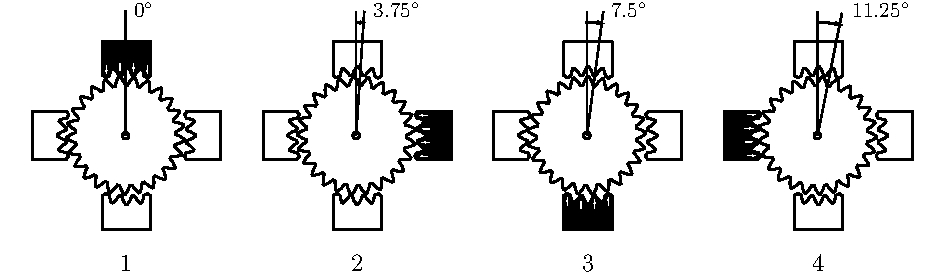
\includegraphics[width=1\textwidth]{diagrams/stepperMotor.pdf}
					\caption{Stepper motor operation}
					\label{fig:stepperMotor}
				\end{figure}
				
			\subsubsection{Extruder}
				
				The extruder consists of a simple DC motor and gearbox which forces
				filament into a heater and out through a nozzle (figure
				\ref{fig:extruder}). There is also a temperature sensor in the heater
				which allows specific temperatures to be maintained.
				
				\begin{figure}
					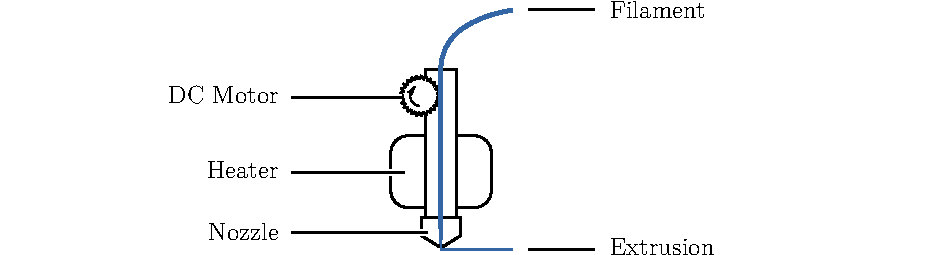
\includegraphics[width=1\textwidth]{diagrams/extruder.pdf}
					\caption{Extruder components}
					\label{fig:extruder}
				\end{figure}
				
			\subsubsection{Platform}
				
				The platform contains a heater which heats the build surface during
				printing. This helps to prevent warping and improve the adhesion of the
				print to the build surface. This heater also contains a temperature
				sensor to allow specific temperatures to be maintained.
				
				The build surface consists of a conveyor belt which is used to eject
				printed objects from the platform after printing completes. The conveyor
				is powered by a small DC motor with a gearbox.
				
		\subsection{Electronics}
		
			The Makerbot is controlled by the RepRap's generation 3 electronics. These
			consist of:
			\begin{description}
				
				\item[Motherboard] This board hosts a microcontroller which communicates
				with a computer and controls the printer's components.
				
				\item[Extruder Controller] This board hosts a second microcontroller
				along with electronics for the extruder motor and temperature sensors.
				The extruder controller communicates with the motherboard via a custom
				RS485-based interface.
				
				\item[Relay Board] This board contains a mechanical relay for each of
				the two heaters to allow them to be powered on and off. The relay board
				is driven by the extruder controller using simple digital signals.
				
				\item[Stepper Motor Driver ($\times 3$)] Boards which produce the
				high-power signals required to drive the stepper motors. These boards
				are connected to the motherboard via a simple digital interface that
				hides messy details of driving a stepper motor.
				
			\end{description}
			
			% TODO: Future generations?
		
	\section{Firmware}
		
		The firmware on the microcontrollers is responsible for two main tasks:
		receiving print data from a computer and producing the signals required by
		the printer to complete the required print job. The signals it generates
		have strict `real-time' timing requirements and so the firmware is required
		to use the specialised timing features of the microcontroller.
		
		3D printers typically receive print data in the form of G-code. G-code is
		the de facto standard for controlling computer numerical control (CNC)
		machines such as 3D printers, laser cutters and CNC lathes. The language is
		human readable and allows step-by-step instructions for machine actions to
		be specified such as `move to (X,Y,Z)' or `enable heater'. Various tools
		exist which can generate G-code instructions for a given 3D model.
		
		The electronics are designed to use the RepRap generation 3 firmware on the
		motherboard and extruder controller. This firmware uses a custom serial
		protocol to communicate with the host computer. This protocol is designed to
		be simple for the microcontroller to use and, amongst various diagnostic
		features, allows simple movement commands to be sent to the printer. G-code
		print data must be converted into this alternative command format in order
		to drive the printer.
	
	\section{Microcontrollers}
		
		The generation 3 electronics use a pair of Arduino-compatible
		microcontrollers to drive the printer. These devices have a fairly minimal
		8-bit instruction set, limited amounts of memory (4KB of RAM) and a very
		limited set of options for high-speed communications. A faster
		microcontroller is needed to solve the problems discussed in
		\S\ref{sec:aims}.
		
		\subsection{ARM \& Mbed}
			
			As well as the high-performance processors designed by ARM for phones, ARM
			also design the Cortex-M series of microcontrollers. For this project the
			Cortex-M3 based Mbed microcontroller was chosen.
			
			\subsubsection{Mbed}
				
				The Mbed is a small microcontroller prototyping board centred around the
				NXP LPC1768, ARM Cortex-M3 based microcontroller (figure
				\ref{fig:mbed}). It has has four debugging LEDs, a USB port for loading
				programs and an interface suitable for attaching an Ethernet port. The
				pins on the bottom of the device expose the LPC1768's input and output
				capabilities and fit into standard, easily soldered 0.1" connections.
				
				\begin{figure}
					
\includegraphics[width=1\textwidth]{diagrams/mbed.pdf}
					\caption{Mbed microcontroller}
					\label{fig:mbed}
				\end{figure}
				
				The Mbed provides a USB flash drive like interface. This interface is
				used to program the device by simply copying binaries on to it as files.
				This mechanism is used to support the device's unusual choice of purely
				web-based tools. This design means no extra software is required for
				development. Web-based development is not ideal for this project and an
				alternative solution is discussed in \S\ref{sec:compiler} to allow
				conventional development tools to be used.
			
			\subsubsection{NXP LPC1768}
				
				The LPC1768 microcontroller behind the Mbed is built around the
				ARM Cortex-M3 processor and provides various useful peripherals. ARM
				devices are extremely widely used and mature open source tools are
				available to develop for the platform.
				
				The LPC1768 runs at up to $100\MHz$ and has $32\KB$ of ram
				\cite{lpc1768}. While still a seemingly tiny amount compared to even a
				modest smart phone, this is a large amount for a microcontroller without
				the overhead of running a fully-fledged general purpose operating system
				and associated software.
				
				The chip contains various peripherals such as hardware timers, analog
				interfaces and, importantly, fast Ethernet support. These timers will,
				as with the previous microcontrollers, be vital for driving the
				electronics properly. Analog inputs are also needed to interface with
				the electronics. Ethernet support will allow the microcontroller to
				quickly receive detailed print data over the network.
				
				
	\section{Real-Time Operating Systems}
		
		As the firmware consists of various complimentary parts (such as
		communication and control), an operating system was selected to manage the
		interaction between them. Due to the stringent timing and performance
		requirements for the software, a real-time operating system (RTOS) was
		selected.
		
		\subsection{Differences From Non-Real-Time Systems}
			
			Real-time operating systems, like other operating systems, provides a
			scheduler which allows multiple processes to run as if simultaneously and
			facilities for communicating between them. Unlike regular operating
			systems, an RTOS can provide accurate timing guarantees. They also tend to
			be targeted at microcontroller development and are compact and function
			without the need for extra hardware such as a memory management unit
			(MMU).
			
		\subsection{FreeRTOS}
			
			FreeRTOS is a widely used, open-source RTOS designed for use on a range of
			microcontrollers, including Cortex-M3 based devices. The two key features
			of FreeRTOS used by this project are `tasks' and `queues' and these are
			described below.
			
			\subsubsection{Tasks}
				
				A system built on FreeRTOS can be structured in terms of several tasks
				executing in parallel. Tasks are similar to processes or threads on a
				conventional operating system and each task has its own set of
				registers and a stack.
				
				Because the processor can only run one task at once, the FreeRTOS uses
				preemptive scheduling to approximate this behaviour. The current task is
				periodically interrupted by a timer (preempted) and a different task put
				in its place. If tasks are switched fast enough, the system appears to
				run all of them simultaneously.
				
				Tasks may be given different priorities and can be suspended until some
				event occurs such as a timer expiring or a hardware resource becoming
				available. The duration of timed delays or the delay between a resource
				signalling its readiness and the task being executed can be guaranteed
				allowing real-time systems to be developed.
				
			\subsubsection{Queues \& Mutexes}
				
				To provide synchronisation and communication between tasks, FreeRTOS
				provides a queue structure. Queues can be defined which allow data to be
				inserted or removed in a first-in-first-out (FIFO) scheme.
				
				These queues can be safely used without race conditions by multiple
				tasks simultaneously and so are ideal for inter-task communication.
				Because of their safety, they also form the basis for the standard
				parallel programming constructions, semaphores and mutexes, in FreeRTOS.
				
				When accessing a FreeRTOS queue the task may be blocked, for example
				when adding an item to a queue that is already full. FreeRTOS can
				provide timing guarantees on timeouts waiting for these functions to
				complete. It also allows a task's priority to be temporarily raised when
				resumed after a blocking call ensuring it is scheduled as soon as
				possible, reducing the delay before any new data data is processed.
